% =====================================================================
% Slide vấn đáp (khoảng 10 slide, 6–8 phút; KE_HOACH_DU_AN.md mục 16.1).
% Biên dịch bằng XeLaTeX (Overleaf: Menu → Compiler → XeLaTeX), đặt cùng thư mục docs/ với báo cáo
% để dùng chung hình ở docs/report/figures/.
% Mỗi người trình bày một nửa, nhưng ai cũng phải trình bày được toàn bộ.
% =====================================================================
\documentclass[aspectratio=169, 11pt]{beamer}
\usepackage{fontspec}
\setsansfont{TeX Gyre Heros}
\setmainfont{TeX Gyre Termes}
\usepackage{polyglossia}
\setdefaultlanguage{vietnamese}
\usepackage{amsmath, amssymb, booktabs}
\usepackage{tikz}
\usetikzlibrary{arrows.meta}
\graphicspath{{../report/figures/}}
\setbeamertemplate{navigation symbols}{}
\setbeamertemplate{footline}[frame number]
\setbeamercolor{structure}{fg=blue!55!black}

\title{Khai thác tập phổ biến bằng Eclat}
\subtitle{Cài đặt bằng Julia, đánh giá hiệu năng và hai ứng dụng}
\author{Phạm Trần Anh Quân \and Nguyễn Tiến Cường}
\institute{Khai thác dữ liệu và ứng dụng, HCMUS}
\date{}

\begin{document}

\begin{frame}
\titlepage
\end{frame}

% ---------------------------------------------------------------------
\begin{frame}{1. Bài toán và ý tưởng của Eclat}
\begin{itemize}
\item Tìm mọi tập item $X$ có $\sigma(X) = |t(X)| \ge \sigma_{\min} = \lceil \mathrm{minsup} \cdot N \rceil$.
\item Apriori: biểu diễn ngang, sinh ứng viên rồi quét lại CSDL ở mỗi mức.
\item \textbf{Eclat} (Zaki, IEEE TKDE 2000): biểu diễn \textbf{dọc}, mỗi item kèm tidset $t(x)$.
  \[ t(X \cup Y) = t(X) \cap t(Y) \quad\Rightarrow\quad \text{không cần quét lại CSDL} \]
\item Chia dàn tập con thành các \textbf{lớp tiền tố} $[P]$ độc lập, giải từng lớp bằng duyệt từ dưới lên.
\item Chi phí tỉ lệ với số tập phổ biến $\times$ chi phí một phép giao.
\end{itemize}
\end{frame}

% ---------------------------------------------------------------------
\begin{frame}{2. Chạy tay: ví dụ hiệu sách của bài báo ($\sigma_{\min} = 3$)}
\centering
\begin{tikzpicture}[font=\small, x=1.6cm, y=1.1cm,
  tap/.style={draw, rounded corners=1pt, align=center, inner sep=2pt, minimum width=1.3cm},
  loai/.style={tap, densely dashed, draw=gray, text=gray},
  >={Stealth[length=4pt]}]
\node[tap] (A) at (0, 0) {A\\1345};
\node[tap] (C) at (1, 0) {C\\123456};
\node[tap] (D) at (2, 0) {D\\2456};
\node[tap] (T) at (3, 0) {T\\1356};
\node[tap] (W) at (4, 0) {W\\12345};
\node[tap] (AC) at (0, -1.4) {AC\\1345};
\node[loai] (AD) at (1, -1.4) {AD\\45};
\node[tap] (AT) at (2, -1.4) {AT\\135};
\node[tap] (AW) at (3, -1.4) {AW\\1345};
\node[tap] (ACT) at (0, -2.8) {ACT\\135};
\node[tap] (ACW) at (1, -2.8) {ACW\\1345};
\node[tap] (ATW) at (2, -2.8) {ATW\\135};
\node[tap] (ACTW) at (0, -4.2) {ACTW\\135};
\foreach \u/\v in {A/AC, A/AT, A/AW, AC/ACT, AC/ACW, AT/ATW, ACT/ACTW} \draw[->] (\u) -- (\v);
\draw[->, gray] (A) -- (AD);
\node[anchor=west, align=left] at (3.0, -3.3)
  {$t(AC) = t(A) \cap t(C) = 1345$\\ $t(ACT) = t(AC) \cap t(AT) = 135$\\ $AD$: 2 giao dịch $< 3$ $\Rightarrow$ loại\\ Kết quả: đúng 19 tập như bài báo};
\end{tikzpicture}
\end{frame}

% ---------------------------------------------------------------------
\begin{frame}{3. Cài đặt: kiến trúc và 7 phiên bản}
\begin{columns}[T]
\column{0.48\textwidth}
\begin{itemize}
\item Hợp đồng giao diện: \texttt{eclat!(sink, db, minsup, cfg)}; thuật toán đẩy mỗi tập ra qua \texttt{sink}.
\item Đọc/ghi định dạng SPMF; $\sigma_{\min}$ tính \emph{giống hệt} SPMF (kiểm chứng bằng thí nghiệm hộp đen).
\item Julia: multiple dispatch chọn hàm giao lúc biên dịch; \texttt{BitVector} + \texttt{@simd}; không cấp phát trong vòng lặp nóng.
\end{itemize}
\column{0.5\textwidth}
\footnotesize
\begin{tabular}{@{}ll@{}}
\toprule
v0 & cơ bản theo bài báo \\
v1 & + item theo support tăng dần \\
v2 & + dùng lại bộ nhớ đệm \\
v3 & + giao thích nghi (dừng sớm, galloping) \\
v4 & + tidset dạng mảng bit \\
v5 & + mảng tam giác cho tập 2 item \\
v6 & + lai: bit $\to$ chỉ số khi $\sigma < N/32$ \\
\bottomrule
\end{tabular}
\end{columns}
\end{frame}

% ---------------------------------------------------------------------
\begin{frame}{4. Tính đúng: khớp SPMF 100\%}
\begin{itemize}
\item \textbf{15.869} phép kiểm tra tự động, chạy trên cả 7 phiên bản:
  oracle duyệt trâu (200 CSDL ngẫu nhiên), 11 đáp án SPMF, dấu vân tay 5 bộ benchmark.
\item \textbf{E1}: 5 bộ $\times$ 7 mức minsup $\times$ 7 phiên bản = \textbf{245/245 tổ hợp khớp}, khoảng 61 triệu cặp (tập, support).
\item Dấu vân tay: tổng các giá trị băm 64 bit của từng dòng, không phụ thuộc thứ tự dòng.
\item Phát hiện khi kiểm chứng: SPMF \texttt{Eclat} hết bộ nhớ khi mã item là $10^6$; cài đặt của nhóm vẫn chạy đúng.
\end{itemize}
\end{frame}

% ---------------------------------------------------------------------
\begin{frame}{5. Hiệu năng so với SPMF}
\begin{columns}[T]
\column{0.62\textwidth}
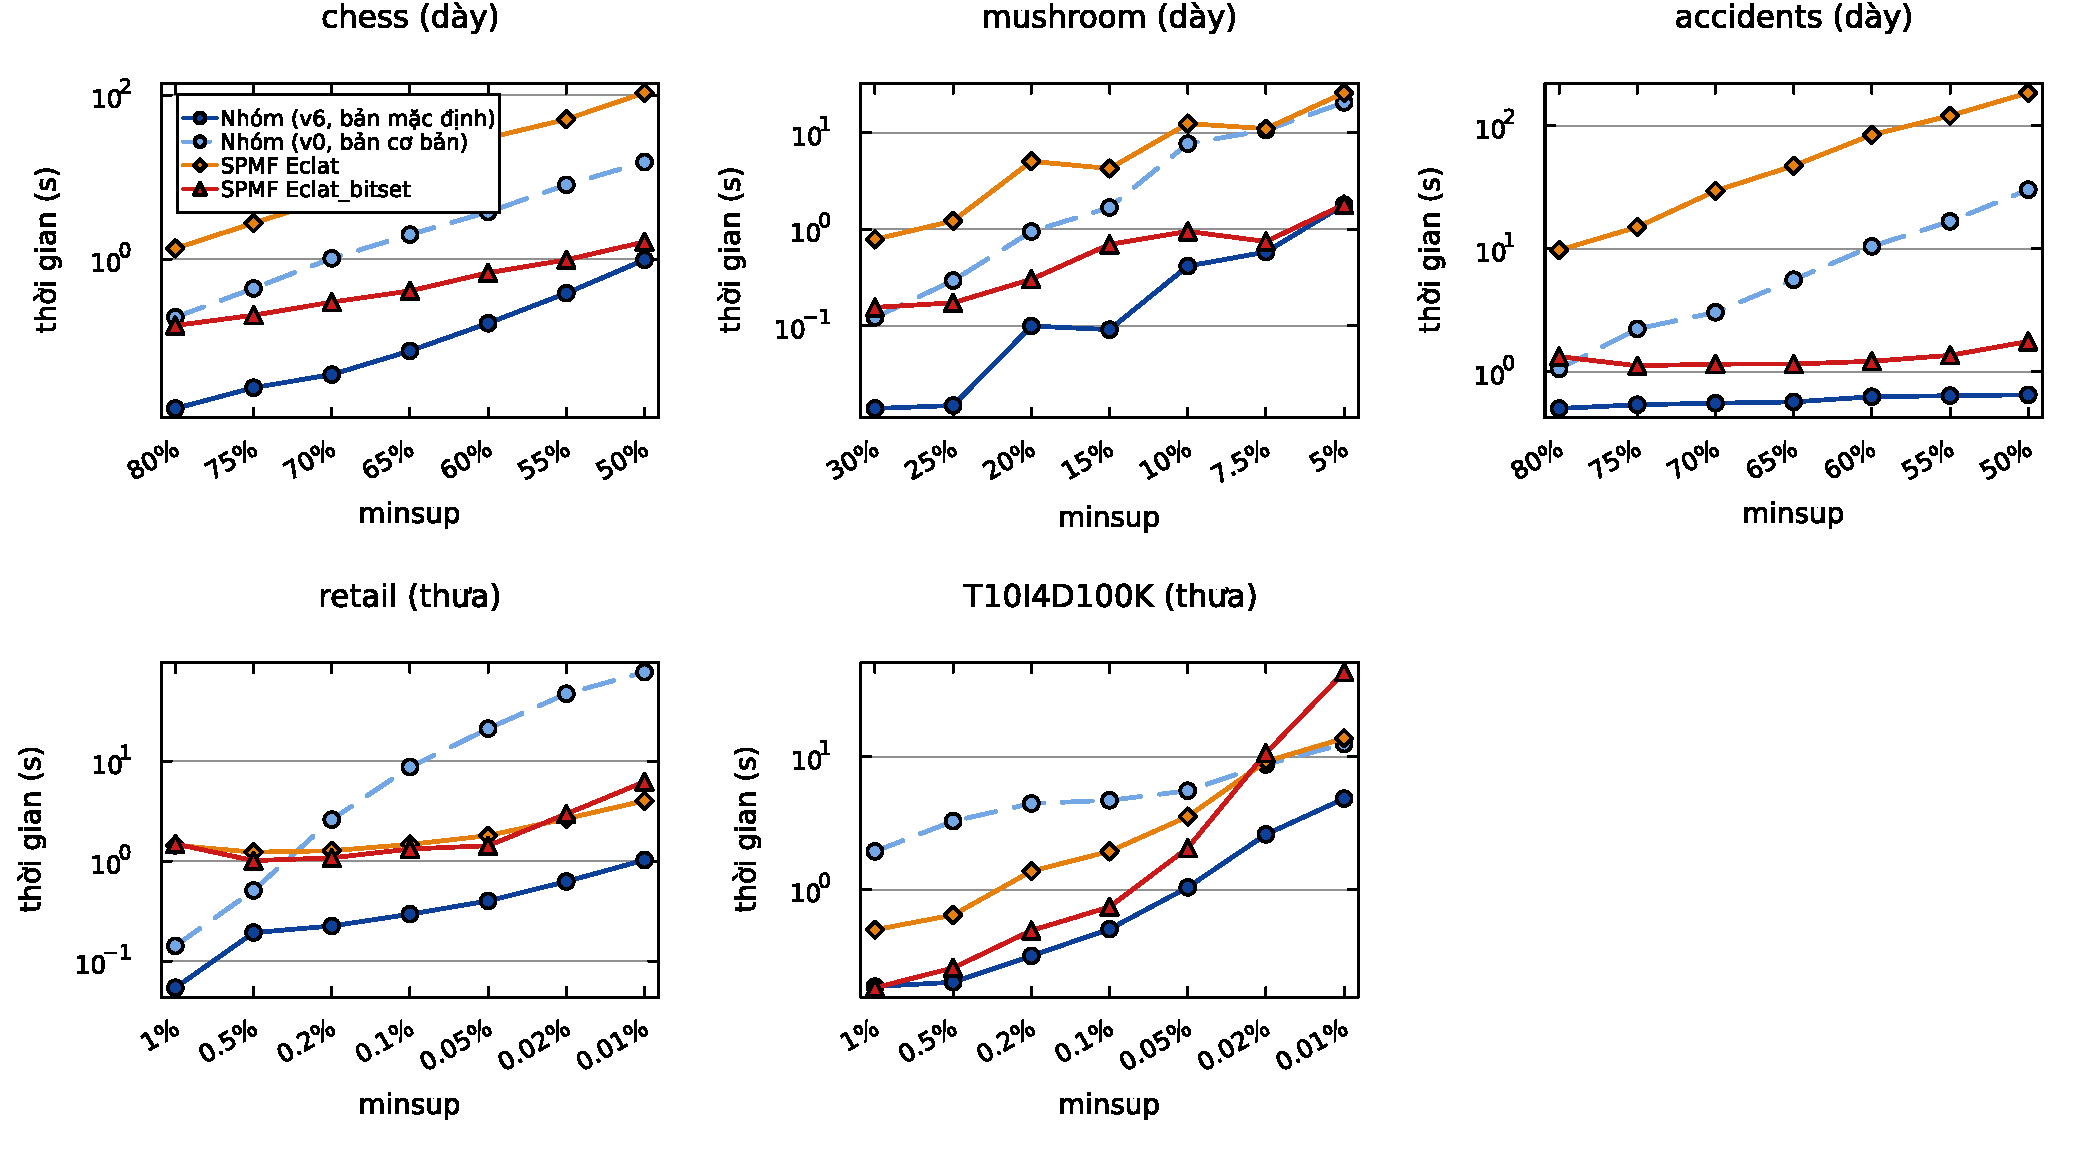
\includegraphics[width=\linewidth]{F03_thoi_gian_theo_minsup}
\column{0.36\textwidth}
\small
\begin{itemize}
\item Thời gian thuật toán: v6 nhanh hơn SPMF \texttt{Eclat} ở 35/35 mức (2,7--285 lần), nhanh hơn \texttt{Eclat\_bitset} ở 34/35 mức.
\item minsup thấp: cả hai bị chặn bởi việc ghi output (v6 chỉ 0,5--0,8\,µs mỗi tập).
\item Thời gian tiến trình: Julia mất 4,5--6\,s khởi động, nên với lần chạy ngắn SPMF xong trước.
\item Mở rộng tuyến tính theo $N$ (Accidents: $R^2 = 0{,}98$).
\end{itemize}
\end{columns}
\end{frame}

% ---------------------------------------------------------------------
\begin{frame}{6. Mỗi tối ưu đóng góp bao nhiêu (ablation)}
\begin{columns}[T]
\column{0.45\textwidth}
\footnotesize
Thời gian (s) ở minsup trung bình\\[2pt]
\begin{tabular}{@{}lrrr@{}}
\toprule
Bản & Chess & Accidents & Retail \\
\midrule
v0 & 2,023 & 5,290 & 10,160 \\
v1 & 1,531 & 1,850 & 6,279 \\
v2 & 0,556 & 0,904 & 5,662 \\
v3 & 0,891 & 0,994 & 2,024 \\
v4 & 0,070 & \textbf{0,081} & 2,360 \\
v5 & 0,065 & 0,235 & \textbf{0,135} \\
v6 & \textbf{0,059} & 0,260 & 0,266 \\
\bottomrule
\end{tabular}
\column{0.53\textwidth}
\small
\begin{itemize}
\item v1: số phép giao giảm 19--49\%.
\item v3: Retail nhanh hơn 2,8 lần (99,8\% phép giao thất bại) nhưng Chess \emph{chậm} hơn 60\%.
\item v4: dữ liệu dày nhanh hơn 10--13 lần.
\item v5: Retail nhanh hơn 17 lần, Accidents \emph{chậm} hơn 2,9 lần.
\item v6: giữ tidset gọn nhưng chậm hơn v5 trên dữ liệu thưa.
\item Nhanh nhất so với v0: 32--75 lần; \textbf{không có bản nào thắng mọi nơi}.
\end{itemize}
\end{columns}
\end{frame}

% ---------------------------------------------------------------------
\begin{frame}{7. Ứng dụng 1: giỏ hàng Groceries}
\begin{itemize}
\item 9.835 hóa đơn, 169 nhóm hàng; minsup 0,5\%, minconf 0,5 $\Rightarrow$ 1.001 tập, 120 luật.
\item Luật mạnh nhất: \{curd, tropical fruit\} $\Rightarrow$ \{yogurt\}, lift 3,69.
\item 9/10 luật đứng đầu có vế phải \emph{other vegetables}: hành vi ``đi chợ nấu ăn''.
\item Xếp theo confidence thì 9/10 luật là ``\dots $\Rightarrow$ whole milk'' (sữa có trong 25,6\% hóa đơn) $\Rightarrow$ phải xếp theo lift.
\item Ổn định: 127/127 luật tìm trên 80\% dữ liệu vẫn có lift $> 1$ trên 20\% còn lại.
\end{itemize}
\end{frame}

% ---------------------------------------------------------------------
\begin{frame}{8. Ứng dụng 2: mẫu trực quan trên ảnh (Caltech-101)}
\begin{columns}[T]
\column{0.58\textwidth}
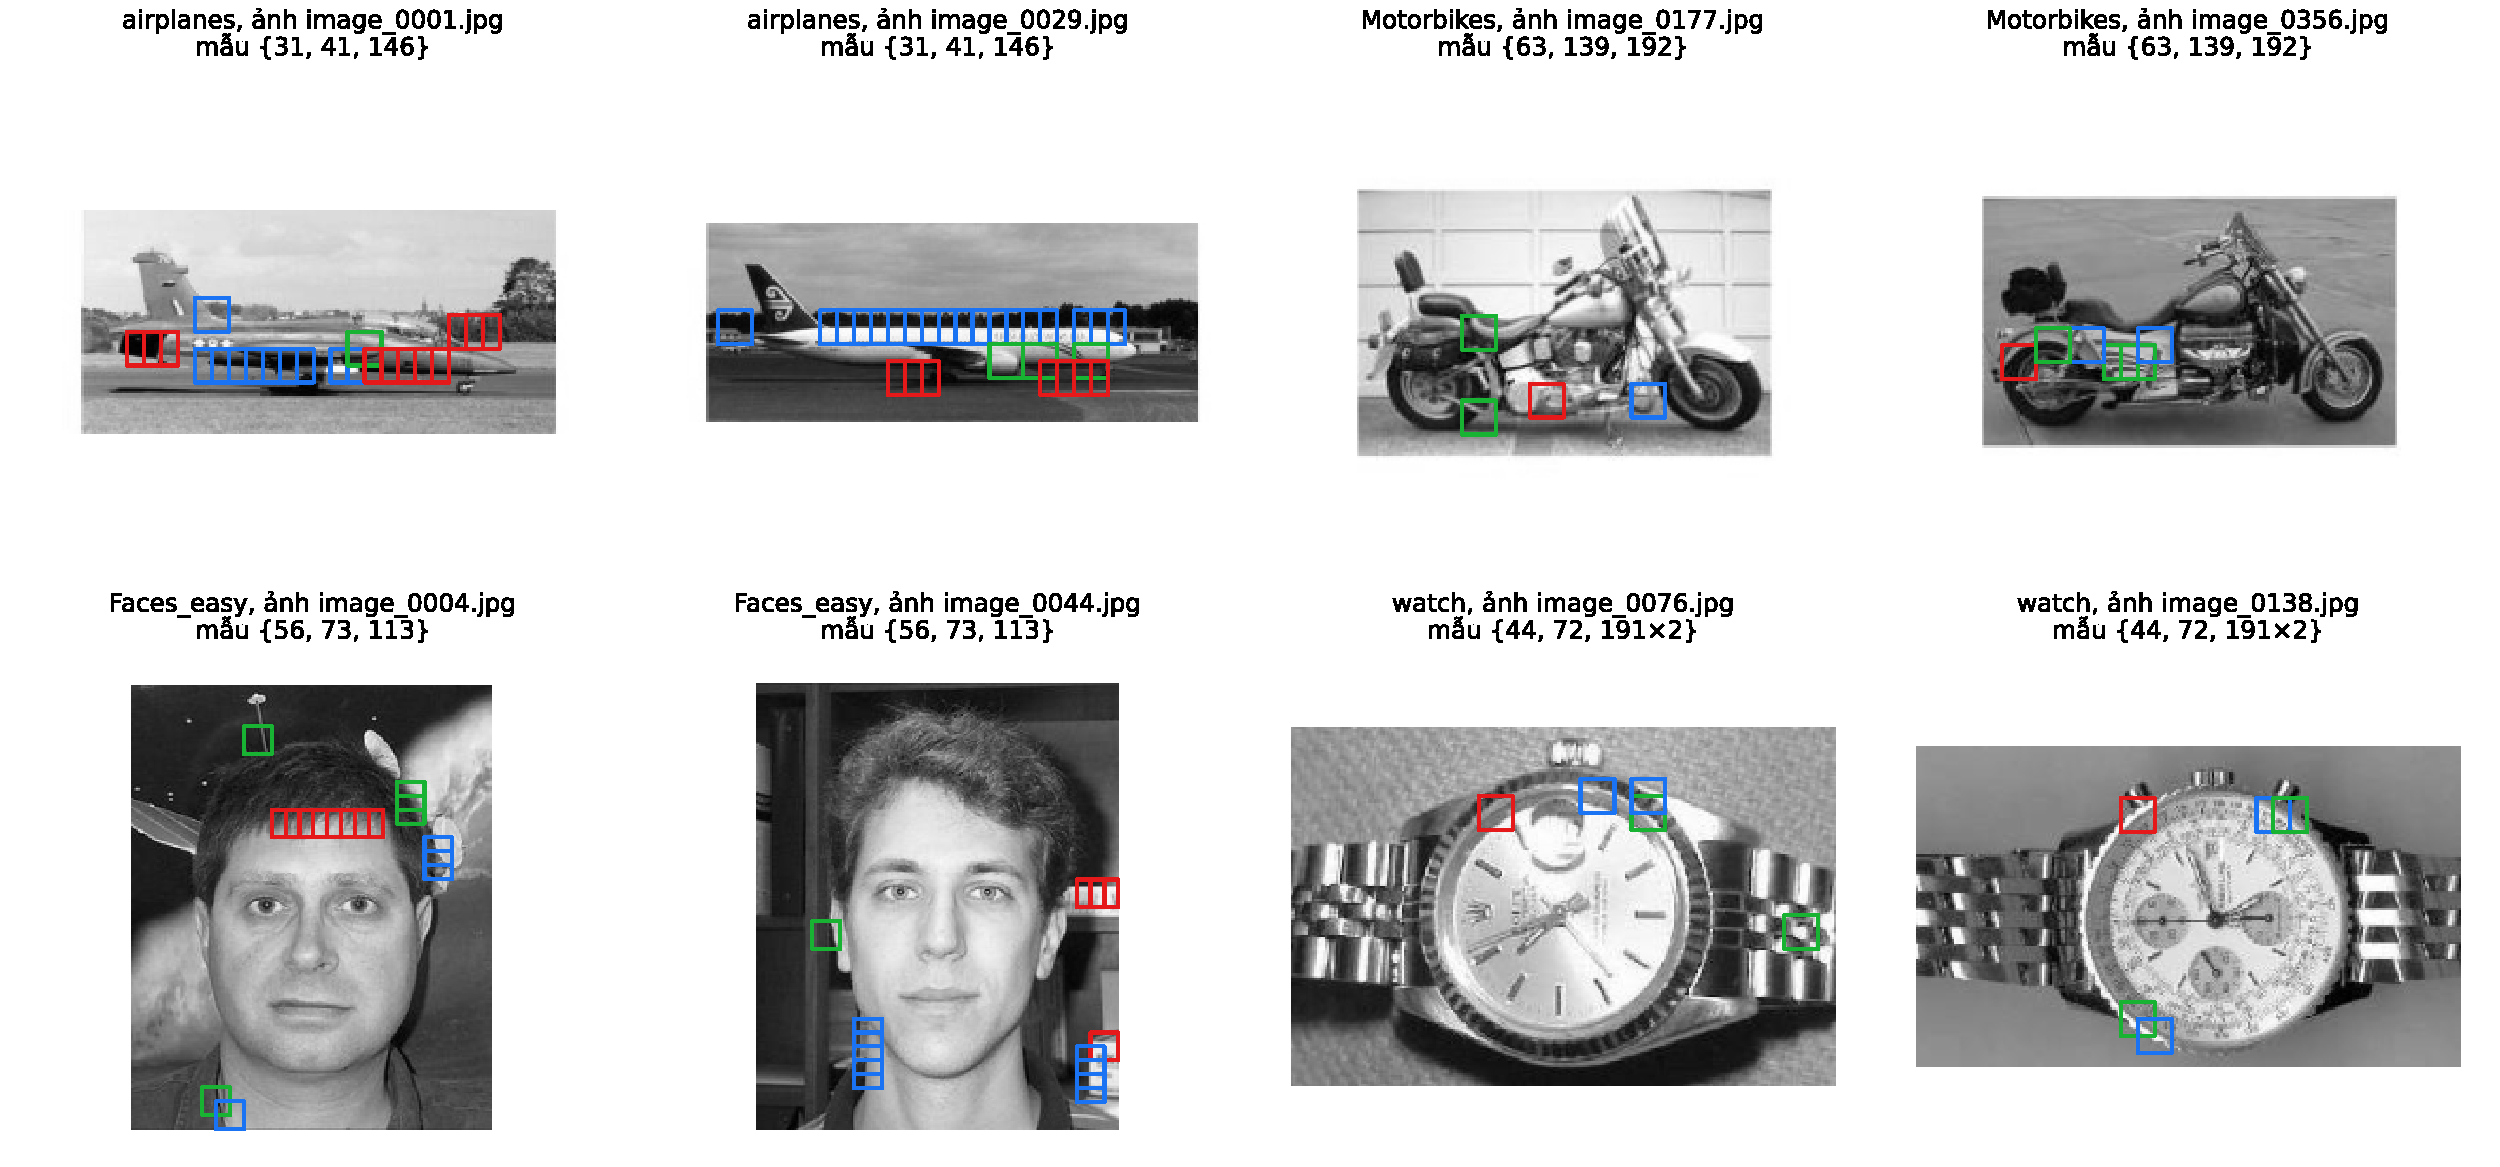
\includegraphics[width=\linewidth]{F12_mau_truc_quan_tren_anh}
\column{0.4\textwidth}
\small
\begin{itemize}
\item Ảnh $\to$ giao dịch các từ thị giác ($k = 200$, có thêm item ``xuất hiện $\ge 2$ lần'').
\item Mẫu đặc trưng mỗi lớp xếp theo tỉ lệ tăng $GR$.
\item Mẫu làm đặc trưng: 75,8\% (80 chiều); kết hợp histogram: 86,7\%.
\item Mẫu của \emph{Faces\_easy} nằm cả trên phông nền: lộ thiên lệch của dữ liệu.
\end{itemize}
\end{columns}
\end{frame}

% ---------------------------------------------------------------------
\begin{frame}{9. Kết luận và hướng tối ưu tiếp theo}
\begin{itemize}
\item Đúng: khớp SPMF 100\% (245/245 tổ hợp, 15.869 phép kiểm tra).
\item Nhanh: thời gian thuật toán nhanh hơn SPMF ở gần như mọi điểm đo; điểm yếu là khởi động Julia.
\item Dự đoán được kiểm chứng: H1, H3, H4, H5 đúng; H2, H8 chỉ đúng một phần; H7 sai, và mỗi chỗ lệch đều giải thích được bằng số đo.
\item Hướng tối ưu tiếp theo:
  \begin{enumerate}
  \item chọn biểu diễn tidset theo mô hình chi phí thời gian;
  \item PrecompileTools.jl để giảm thời gian khởi động;
  \item diffset (dEclat) cho dữ liệu dày;
  \item song song hóa các lớp ở mức 1.
  \end{enumerate}
\end{itemize}
\end{frame}

\end{document}
